\section{Odraz míčku}
\label{sec:odraz-micku}

Samotný odraz je pro tuto práci nejdůležitější. Tedy bude probrán velmi
podrobně. Důležitým předpokladem je, že \speed{1} a \spin{1} jsou hodnoty přímo
před odrazem. Díky tomuto předpokladu nemusíme uvažovat let míčku
popsaný v \myref{sekci}{sec:let-micku} ani jeho letové vlastnosti.

Problém je i tak stále velmi komplexní, protože na odraz má vliv hned několik
proměných. Ty společně s charakteristikou celé odrazové periody budou popsány v
této sekci.

Obecně se všechny proměné v tomto problému dají rozřadit do tří kategorií:

\begin{description}
 \item[Nezávislé] Pro tuto práci to jsou: \speed{1},~\spin{1} a \angle{1}.
 \item[Závisé] Analogicky se jedná o: \speed{2},~\spin{2} a \angle{2}.
 \item[Kontrolované] Jde především o materiálové konstanty:
  verikální/horizontální koeficient restituce ($e_{y/x}$), koeficient smýkavého
 tření ($\mu$), poloměr ($R$), koeficient momentu hybnosti ($\alpha$),
 vzdálenost geometrického středu od působení normálové síly ($D$).
\end{description}

Závislé a nezávislé proměné jsou znázorněné na \myref{obrázku}{fig:odraz-micku}.
Nezávislé jsou proměné před odrazem a na nich závisí proměné po odraze.
Kontrolované proměné na \myref{obrázku}{fig:odraz-micku} nejsou, ale stále je
důležité je uvést pro replikovatelnost výsledků. Také budou z pravidla přebírány
z odborné literatury, a tedy nebudou mnou měřené. 

\begin{figure}[htbp]
 \centering
 \documentclass{article}
\usepackage{tikz}
\usepackage{xcolor}
\usepackage{mathtools}

\definecolor{darkgreen}{rgb}{0.0,0.5,0.0}
\begin{document}

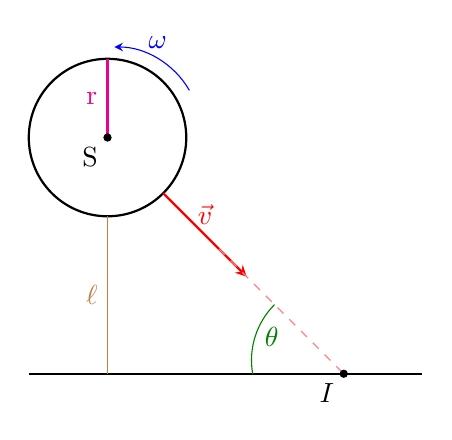
\begin{tikzpicture}
	%ball
	\draw[thick] (0,0) circle (1);
	%radius
	\draw[magenta,thick] (0,0) --node[midway,left] {r}++ (0,1);
	\node[fill=black,circle,inner sep=0pt, minimum size=3pt](s) at (0,0) {};
	%center
	\node[below left](slabel) {S};

	%speed
	\draw[red,thick,-stealth](-45:1) --node[above] {$\vec{v}$}++ (-45:1.5);
	\draw[red!50,dashed](-45:2) -- (-45:4.3);

	%graund
	\draw[thick] (-1,-3) -- (4,-3);

	%vercial length
	\draw[brown] (0,-1) --node[left] {$\ell$}++ (0,-2);

	%angle
	\node[fill=black,circle,inner sep=0pt, minimum size=3pt](naraz) at (3,-3)
	{};
	\node[below left] at (naraz) {$I$};

	\draw[darkgreen] (-45:3) arc[
			start angle = 135,
			end angle = 190,
			radius = 1,
		] node[midway,right] {$\theta$};

	%angular velocity
	\draw[blue,-stealth] (30:1.2) arc(30:90:1.1) node[midway,above] {$\omega$};
\end{tikzpicture}
\end{document}



 \caption{Síly a veličiny působící na míček při odrazu}
 \label{fig:odraz-micku}
\end{figure}

\subsection{Koeficienty restituce}
\label{ssec:koeficienty-restituce}
elasticita odrazu 

\subsection{Moment hybnosti}
\label{ssec:moment-hybnosti}
jak moc Déčko reálně ovlivňuje spin

\subsection{Tření po dobu odrazu}
\label{ssec:treni-po-dobu-odrazu}
otačí se podle toho jestli převládá spin nebo speed


